\documentclass[12pt, a4paper]{article}

\usepackage [utf8]{inputenc}
\usepackage [IL2]{fontenc}
\usepackage [czech]{babel}
\usepackage{graphicx}
\usepackage[numbib]{tocbibind}
\usepackage{hyperref}
\graphicspath{{obrazky/}}
\newcommand{\Break}{\State \textbf{break} }

\title{
\includegraphics[width=10cm]{FAV_cmyk}

{\huge Semestrální práce z KIV/TI}

\vspace{0.5cm}
{\LARGE Logické řízení - sanitace nádrží}
\vspace{1cm} 

\Large Lukáš Runt (A20B0226P)

\large {\itshape lrunt@students.zcu.cz}

\vspace{0.1cm}
\Large Miroslav Vdoviak (A20B0268P)

\large \itshape{miravdov@students.zcu.cz}
}
\date{\vspace{6cm} \today}

\begin{document}

\begin{titlepage}
\clearpage\maketitle
\thispagestyle{empty}
\end{titlepage}
\tableofcontents \newpage

\section{Zadání}
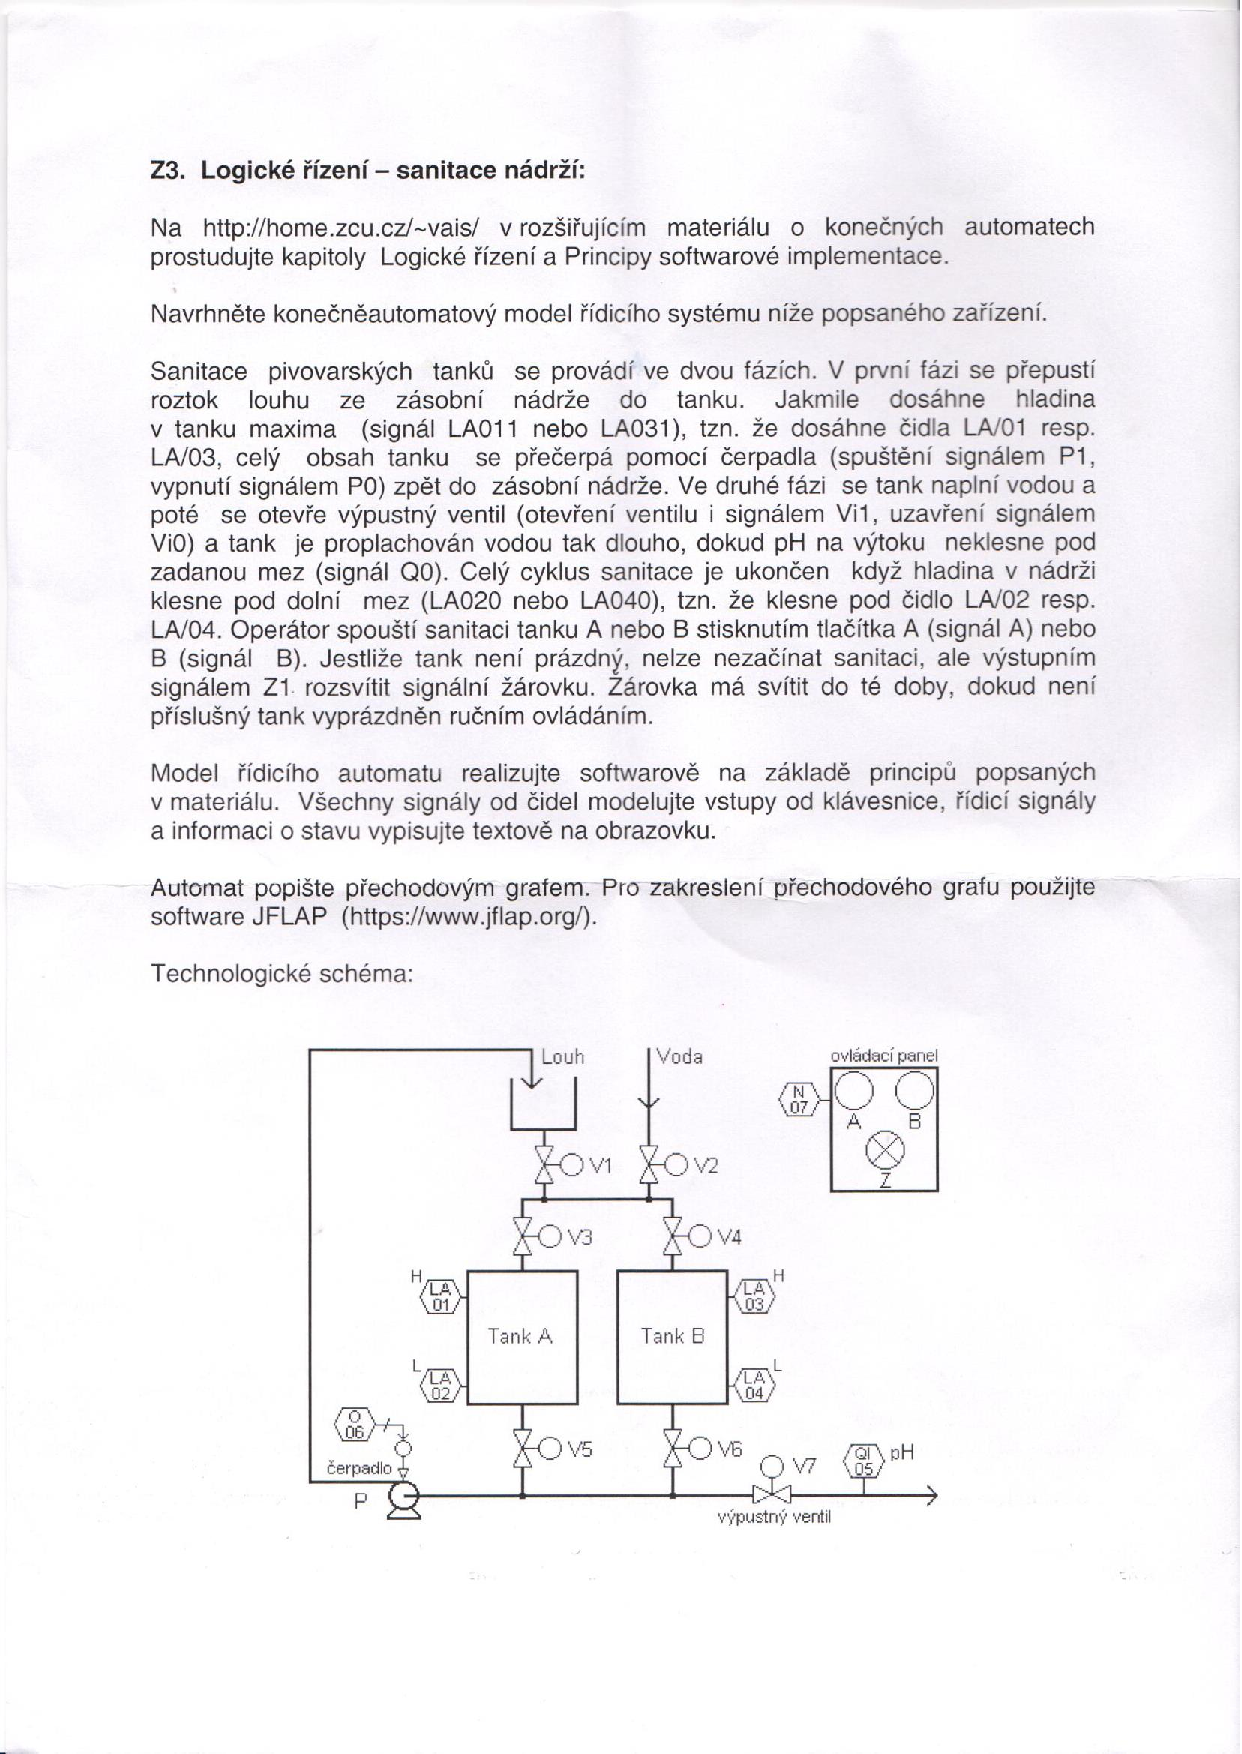
\includegraphics[width=14cm]{TI.pdf}

\section{Analýza úlohy}

\section{Automatový model}

\subsection{Stavy}
STAV 0 - Systém není v činnosti \newline 
STAV 1 - Tank A se napouští lihem \newline 
STAV 2 - Tanku A se přečerpává čerpadlem \newline 
STAV 3 - Tank A se plní vodou \newline 
STAV 4 - Tank A se proplachuje dokud není ph v normálu \newline 
STAV 5 - Tank A se vypouští \newline 
STAV 6 - Tank B se napouští lihem \newline 
STAV 7 - Tanku B se přečerpává čerpadlem \newline 
STAV 8 - Tank B se plní vodou \newline 
STAV 9 - Tank B se proplachuje dokud není ph v normálu \newline 
STAV 10 - Tank B se vypouští 

\subsection{Snímače}
LA011 - Hladina dosahuje maxima tanku A \newline 
LA010 - Hladina nedosahuje maxima tanku A \newline 
LA021 - Hladina dosahuje minima tanku A \newline 
LA020 - Hladina nedosahuje minima tanku A \newline 
LA031 - Hladina dosahuje maxima tanku B \newline
LA030 - Hladina nedosahuje maxima tanku B \newline 
LA041 - Hladina nedosahuje minima tanku B \newline 
LA040 - Hladina dosahuje minima tanku B

\subsection{Řídící signály}
P0 - Čerpadlo vyplé \newline 
P1 - Čerpadlo zaplé \newline 
Vi0 - Ventil i zavřen \newline 
Vi1 - Ventil i otevřen \newline 
Q0 - Ph nad požadovanou mezí \newline 
Q1 - Ph pod požadovanou mezí 

\subsection{Řízení operátora}
A - Sanitace tanku A \newline 
B - Sanitace tanku B \newline 
Z - Žárovka

\subsection{Přechodový graf}
Na naásledujícím obrázku je přechodový graf konečného automatu.
\begin{figure}[h]
\centering 
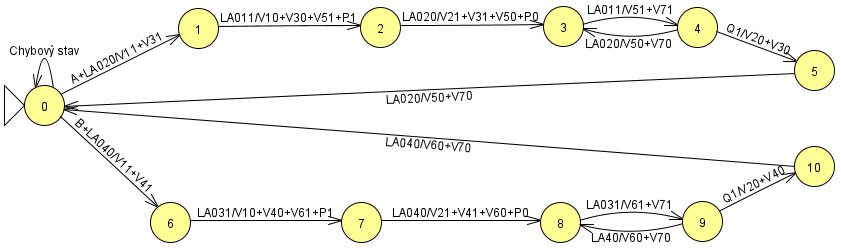
\includegraphics[width=14cm]{prechodovyAutomat}
\caption{Přechodový graf automatu}
\end{figure}

\subsection{Chybové stavy} \label{chyba}
\begin{itemize}
  \item Uživatel chce začít sanitarizaci tanku, který není prázdný
  \item Uživatel chce začít sanitarizaci tanku v době, kdy se sanitarizuje jiný tank
  \item Uživatel chce míchat líh s vodou
  \item Uživatel chce vylévat líh do potrubí
  \item Uživatel chce čerpat vodu do nádrže s lihem
\end{itemize}

\section{Implementace}
Program je implementován v jezyce Java. Při vytváření programu bylo zvažováno, zda nebudou nakresleny obrázky v nějakém z grafických editorů, které se budou postupně měnit. Toto nám, ale přišlo krajně nepraktické, a proto byla zvolena implementace s pomocí knihovnou \texttt{Java Swing} a vektorovou grafikou, která se bude překreslovat podle aktuálního stavu. 

\vspace{0.25cm}
Tato knihovna vytváří okno v metodě \texttt{main()}, které má pevně stanovenou velikost. O obsah okna se stará třída \texttt{DrawingPanel}, která je zodpovědná o vzhled modelu. Tato třída obsahuje i logiku automatu. Při spuštění se vše inicializuje tak, aby se vykreslil automat ve stavu 0, tedy v nečinnosti.

\vspace{0.25cm}
Každá komponenta má svoji proměnnou, která uchovává její stav. Tento stav se poté promítá do výsledného grafického výstupu. Stavy komponent jsou reprezentovány barvami. Zelená znamená logickou 1 a červená logickou 0. Toto neplatí u žárovky, která je při logické 1 žlutá a při logické 0 šedá. Komponenta tanku je pak řešena tak, že uchovává data o její plnosti v procentech a druh jejího obsahu (voda, líh, vzduch), který je řešen pomocí enumu \texttt{Napln}.

\vspace{0.25cm}
Stavy modelu jsou realizovány pomocí proměnné \texttt{stav} datového typu \texttt{Integer}. V programu je zabudovaný \texttt{timer}, který každých \texttt{50ms} spustí matodu \texttt{zjistiStav()}, která zjistí stav a následně podle toho spustí metodu příslušející aktuálnímu stavu modelu. Každý stav pak vykonává nějakou pro něj typickou činnost (plnění tanku, čerpání lihu z nádrže, atd.), dokud není splněna podmínka (např.: pro stav 1 snímač LA01 je v logické 1), pokud je potřebná podmínka splněna, model se přesouvá do dalšího stavu (uložení do proměnné \texttt{stav} příslušné hodnoty). metody stavů jsou nazvány \texttt{stav[A|B][1|2|3|4|5]}. Pro aktualizování stavu snímaču slouží metoda \texttt{aktualizujStav()}, která kontroluje, zda má smímač posílat logickou 1 nebo 0.

\vspace{0.25cm}
Reakce na uživatele je vyřešena pomocí metody \texttt{keyListener()}, rozeznávající, která klávesa byla stisknuta nebo uvolněna. Díky této metodě lze spoštět jednotlivé sanitarizace a manuálně ovládat model, avšak manuální ovládání je povoleno jen, když je konečný automat ve stavu 0. K zjištění, zda je ovládání povoleno slouží metoda \texttt{isManualniPovoleno()}. Jestliže chce uživatel spustit akci, která nemůže být spuštěna z důvodu chybového stavu, je zavolána metoda \texttt{vypisChybu()}, která vypíše ve vyskakovacím okně chybu a rozsvítí žárovku, která zhasne po zavření okna, které se zobrazilo.

\section{Uživatelská příručka}

\subsection{Spuštění programu}
Aplikace se spoští pomocí příkazu v příkazové řádce. Před zadáním příkazu se musíme ujistit, zda se nacházíme ve stejné složce, jako jar soubor, který se chystáme spustit (\texttt{semestralkaTI.jar}). Aplikaci poté spustíme pomocí příkazu: \texttt{java -jar semestralkaTI.jar} \ref{spusteni}. Pro spuštění je předpokladem mít nainstalovanou Javu verze nejméně 11. Odkaz ke stažení Javy 11: \url{ https://www.oracle.com/java/technologies/downloads/#java11}

\begin{figure}[h]
\centering 
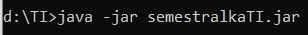
\includegraphics{prikladSpusteni}
\caption{Příklad spuštění}
\label{spusteni}
\end{figure}

Pokud se program podaří spustit zobrazí se model sanitarizace tanků \ref{vzhled}.

\begin{figure}[h]
\centering 
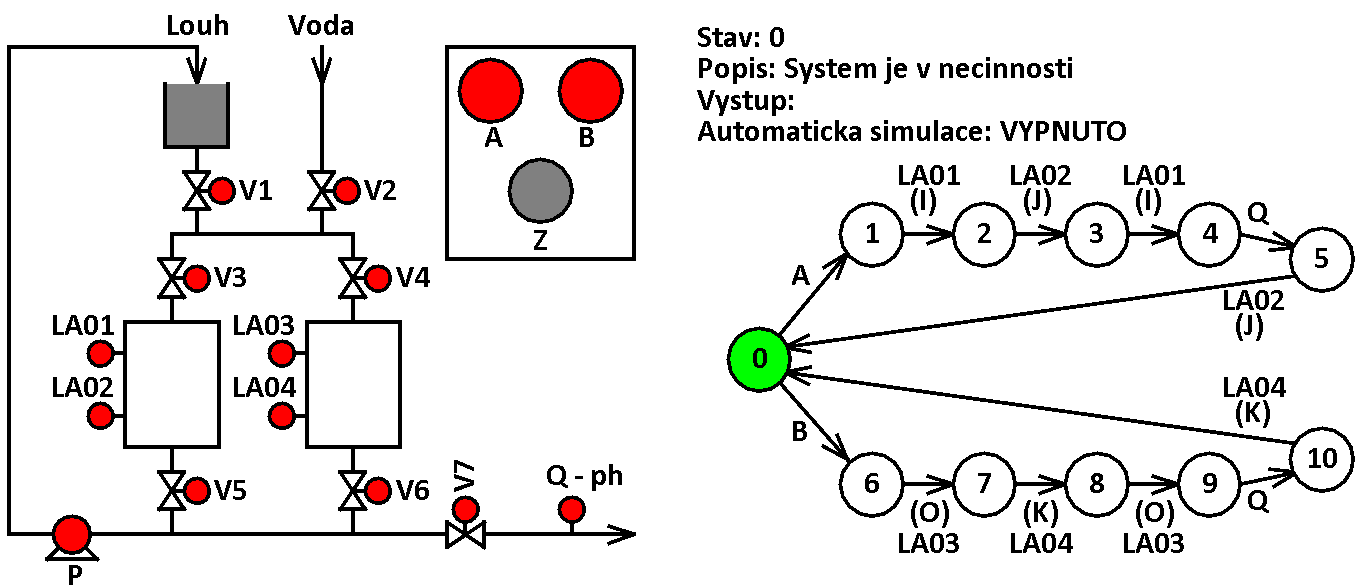
\includegraphics[width=10cm]{pospusteni}
\caption{Vzhled aplikace po spuštění}
\label{vzhled}
\end{figure}

\subsection{Ovládání aplikace}
Po spuštění se zobrazí model ve stavu 0. Červená barva znamená logicloku 0, tedy ventil je zavřené, tlačítko není stlačeno, ph není v požadované mezi, čerpadlo nečerpá líh, hladina v tanku není výš než snímač. Zelená barva znamená naopak logickou 1, tedy ventil je otevřený, tlačítko je stlačeno, atd. Žárovka má své barvy a to šedou pokud nesvítí a žlutou pokud svítí. Voda je znázorněna modrou barvou a líh barvou šedou.

Aplikace se ovládá pomocí klávesnice. Uživatel má k dispozici ovládací panel (Spouštění sanitarizace nádrží) a manuální ovládání, které zahrnuje ovládání jednotlivých ventilů a čerpadla. Při implementaci byla snaha o intuitivní ovládání, tedy ventily se ovládájí pomící jejich čísla, ostatní prvky se ovládají pomocí písmenka, kterým je daný prvek pojmenovaný. Podrobný výčet ovládání je uveden níže \ref{ovladani}.

Aplikace počítá s neobvyklým zacházením. Jsou tedy ošetřeny stavy, při kterých by mohlo dojít k chybě. Při chybovém stavu vyskočí na uživatele upozornění a v modelu se rozsvítí žárovka. Výčet chybových stavů lze najít zde: \ref{chyba}

\subsubsection{Výčet ovládacích kláves} \label{ovladani}
A - Spuštění sanitarizace tanku A \newline 
B - Spuštění sanitarizace tanku B \newline 
P - Manuální spuštění čerpadla \newline 
1 - Manuální otevření ventilu 1 \newline 
2 - Manuální otevření ventilu 2 \newline 
3 - Manuální otevření ventilu 3 \newline 
4 - Manuální otevření ventilu 4 \newline 
5 - Manuální otevření ventilu 5 \newline 
6 - Manuální otevření ventilu 6 \newline 
7 - Manuální otevření ventilu 7 \newline 

\section{Závěr}
Celkovou práci hodnotím pozitivně, neboť se nám povedlo zprovoznit model sanitarizace pivních tanků. V rámci úlohy jsme si vyzkoušeli napsat konečný automat. Byl to pro nás zážitek, který nás studijně obohatil a posunul o krok blíže k praktickým aplikacím teoreticky získaných vědomostí. 

\end{document}